The noisy data have proved to be full of interesting information: they have showed universal behaviors among object-oriented programming languages but they also highlight structural differences in inheritance management.

%Models are useful allies in data analysis. The mean field model allows an interpretation 
%
\subsubsection{Hierarchical sizes distribution is universal}
%The scale-free power law seems to be the dominant distribution of every main quantity obtained from data and the exponents are almost universal.
Hierarchies sizes distribution is power law distributed and there are no differences among the three programming languages.

\subsubsection{The speciation of classes has a universal behavior}
Despite the differences among C++, Java and Python, the speciation is used in the same way, and so the distribution of the number of classes that inherits code from a selected class is the same.

\subsubsection{Multiple inheritance is ever less used than speciation}
The multiple inheritance is used with differences between the three languages. It is always used less than speciation, even in Java, where it has a different and more useful meaning.

\subsubsection{Hierarchies are shallow}
The vast majority of graphs have a depth equal to two or three while the deepest hierarchies have at most a depth of about eleven, or twelve.

\subsubsection{Java hierarchies are shallower}
Java hierarchies show a depth sistematically lower than the Python and C++, while graph sizes behave in the same way.

\subsubsection{The depth is a logarithmic function of the hierarchy size}
In C++ and Python, the mean of depths of hierarchies as a function of the number of classes has a logarithmic behavior.

\subsubsection{Huge hierarchies behave differently}
The depth of huge hierarchies doesn't fit the logarithmic behavior of small and medium hierarchies. It is systematically over such function.

\subsubsection{Speciation is a function of levels}
Classes that does lots of speciation are always at the higher levels.

\vspace{1cm}
The Minimal Effort model gives a link between the hierarchical structures and the effort done to build them. It allows to give an interpretation to data, and it is a guide to key quantities.

\vspace{0.5cm}
The Sharing Tree model extends the mean field model and allows Monte Carlo simulations. The mechanism implemented is close to the natural approach of programmers in objects organization and Sharing Monte Carlo trees well reproduce the data hierarchies.

\vspace{0.5cm}
The depth is the central quantity for optimization mechanism, since it governs the hierarchical structures for fixed size and the proportion between the vertical and the horizontal dimension. Programmers seems to follow the advise to keep the depth as shallow as possibile to avoid the yo-yo problem instead of looking for the optimal structure for code reuse.

\vspace{0.5cm}
The optimization resulting from the competition between the reuse and the abstractability of the code seems to play an important role in the construction of hierarchical inheritance structures in object-oriented programming languages.


\comment{
 caused by the different rules chosen by Java designers.

Java designers have obtained one of their proposals: Java hierarchies are sistematically shallow then C++ and Python ones.


Il numero di oggetti che compongono le strutture gerarchiche ha una
distribuzione a potenza, sostanzialmente universale rispetto ai tre linguaggi
di programmazione analizzati.


In particolare, il linguaggio di programmazione Java presenta strutture
sistematicamente meno profonde rispetto agli altri due linguaggi presentati.
Questo ed altri comportamenti anomali sono frutto di alcune importanti
differenze nella gestione dell’ereditariet`a decise dagli ideatori del linguaggio
Java e con l’obiettivo di minimizzare la complessit`a strutturale del codice,
obiettivo che grazie all’analisi dati possiamo dichiarare raggiunto sotto molti
aspetti.

L’osservazione critica dei dati attraverso le previsioni del modello mean
field propone un primo risultato interessante: le gerarchie appaiono meno
profonde di quelle ottimali. Nei dati si evince infatti che l’outdegree medio
`e generalmente una quantit`a decrescente come funzione della distanza dalla
radice, trend che viene interpretato dal modello come un regime non ottimale
a causa di una profondit`a troppo bassa. Questo risultato `e altres`ı confermato
da generali istruzioni che in ambito informatico suggeriscono di limitare la
complessit`a delle gerarchie in funzione di un pi`
u semplice utilizzo delle stesse.

La previsione dell’andamento dell’outdegree medio come funzione del-
la distanza dalla radice nel modello Sharing Tree risulta una funzione ben
sovrapponibile all’effettivo comportamento delle gerarchie nei linguaggi di
programmazione.

Altre quantit`a nei dati sono risultate in pieno accordo con i modelli,
come ad esempio la profondit`a delle strutture come funzione del numero di
oggetti della gerarchia che si presenta in buona approssimazione logaritmica,
comportamento previsto da entrambi i modelli.



%\begin{figure}[ht]%
%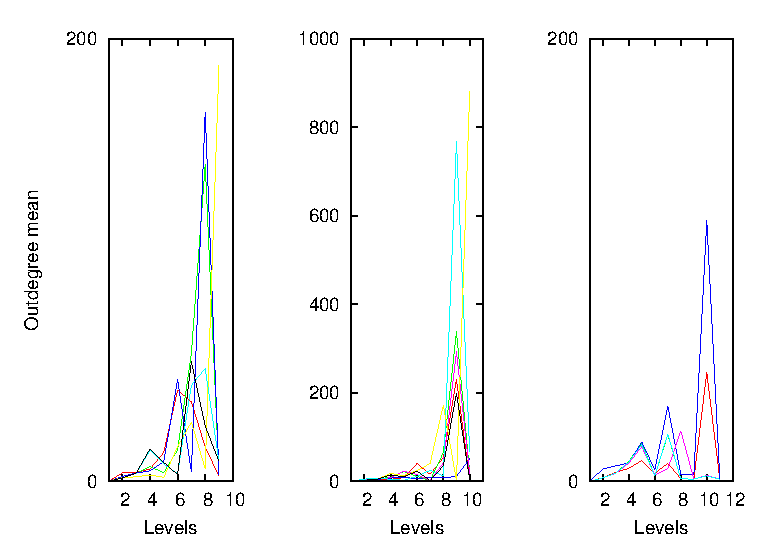
\includegraphics[width=\textwidth,draft=false]{grafici/Coutdeg.cpp1.eps}
%\caption{\label{Foutdeg} \footnotesize\textbf{Cpp} - Very beautiful.}
%\end{figure}


}
